\documentclass[12pt]{article}

%-------Packages---------
\usepackage{amssymb,amsfonts}
\usepackage{enumerate}
\usepackage[margin=0.75in]{geometry}
\usepackage{rotating}
\usepackage{amsthm}
\usepackage{booktabs}
\usepackage{float}
\usepackage{listings}
\usepackage[parfill]{parskip}

\newtheorem{theorem}{Theorem}
\newtheorem{lemma}{Lemma}
\newtheorem{proposition}[theorem]{Proposition}
\newtheorem{corollary}[theorem]{Corollary}
\newenvironment{definition}[1][Definition]{\begin{trivlist}
\item[\hskip \labelsep {\bfseries #1}]}{\end{trivlist}}

%--------Meta Data: Fill in your info------
\title{
  Preventing Leakage of Distribution in Order Preserving Encryption Schemes \\ \vspace*{.3in}
\small Hrishikesh Joshi, Max Kolysh, Mari Miyachi, John Wang \\
\small 6.857 Final Paper \\
\small May 15, 2013}
\date{}

\begin{document}

\maketitle

\abstract{Order Preserving Encryption (OPE) schemes have been heavily studied in the cryptography literature because of their potential application to database design. Unfortunately, few schemes have been able to achieve provable security and leak the minimum amount of information possible. Until Popa et al (2013), no OPE scheme achieved IND-OCPA security. However, even Popa et al's design potentially leaks the distribution of repeated ciphertexts. This paper provides two schemes which are both IND-OCPA secure and do not leak the distribution of ciphertexts. We introduce the notion of IND-CPDA security, and show that both of our schemes satisfy the notion. Finally, we provide experimental results on the effectiveness of these two schemes in practice.}

\newpage

\tableofcontents

\newpage

\section{Introduction}

Order-preserving encryption schemes serve to generate ciphertexts that preserve the numerical ordering of the plaintexts. Such schemes provide an entity for storing encrypted data, such as a mail server or a server interacting with a database, and the ability to perform order comparison operations such as sorting, range query checks, and ranking, among other applications. The ideal security goal for an order-preserving encryption scheme, IND-OCPA, is for the scheme to reveal nothing except for the order of the plaintexts.

For more than a decade, researchers have developed such schemes with varying degrees of success. Often, these schemes compromised security to preserve order, leaking plaintexts or other attributes of the data. Recently, the first order-preserving encryption scheme that satisfies IND-OCPA, mutable order-preserving encoding (mOPE), was proposed by Popa et al (2013). mOPE works by creating a balanced search tree containing all the encrypted data on a server, giving the server the ability to order the tree based on the plaintexts without learning any information regarding the plaintexts themselves. All encrypted values are represented by a node in the balanced search tree. Each node has an Order Preserving Encoding (OPE) which represents its path on the tree from the root to itself, allowing the server the ability to maintain the order of the plaintexts.

One disadvantage of mOPE, however, is that multiple entries of the same plaintext value are maintainted in the same node in the tree with a counter. This means that the scheme can leak information about the distribution of plaintext values. In this paper, we present two schemes that address this issue: Distribution Confidentiality Scheme (DCS) and Random Tiebreaking Order Preservering Encryption (RTOPE). Further, we define a new security guarantee, Indistinguisability Under Chosen Plaintext Distribution Attack (IND-CPDA), which these schemes are intended to satisfy.

To better understand the performance and equivalence of our two schemes, we implemented both with a client-server framework that supports insertion and query functionality. We evaluated the number of OPE re-encodings that resulted over a range of benchmark inputs. These inputs also had varying amounts of repetition, to better evaluate our schemes under uneven plaintext distributions. We show the results of this work, and prove that the two schemes are not structurally expectation equivalent.

The rest of the paper is organized as follows: II discusses mOPE, including related work, III presents DCS, IV describes IND-CPDA, V presents RTOPE, VI compares the two schemes, DCS and RTOPE, VII describes the experimental results of our implementation of the two schemes, and finally VIII concludes with a brief overview of our overall approach. 

\section{Mutable Order-Preserving Scheme (mOPE)}

As mentioned earlier, mOPE is the first known order-preserving scheme that satisfies IND-OCPA, leaking nothing with the exception of the order of the plaintexts. In this section we describe how mOPE works, including the leakage of distribution that it can lead to. We begin with two entities, an untrusted server and a client with confidential data as shown in Figure 1.

\begin{figure}[htb]
\begin{center}
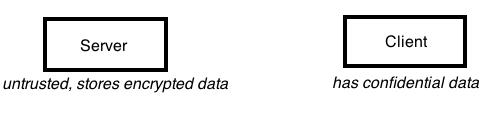
\includegraphics[height=1.2in,width=4in,angle=0]{857pic4.png}
\caption{The client hosts confidential data in encrypted form on the untrusted server. mOPE allows subsequent operations requiring order to be performed on the encrypted data on the untrusted server.}
\end{center}
\end{figure}

\subsection{Storage of Data on Client and Server}

Figure 2 below depicts the data maintained by the client and server at a given point in time. The client hosts confidential plaintext data and and the corresponding ciphertexts. The client relays the ciphertexts to the server, which maintains a table with the corresponding ciphertexts. The B-tree maintained by the server shows the data marked by the ciphertext values, which the server knows, but ordered by the underlying plaintexts, which the server does not know. The ability for the server to maintain such order based on plaintexts without knowing the underlying plaintexts is explained in the next section. It is important to note that the server generates Order-Preserving Encodings (OPEs) for each of the ciphertexts in the B-tree, and preserves a mapping between OPEs and ciphertexts as shown in the table the server maintains.

\begin{figure}[htb]
\begin{center}
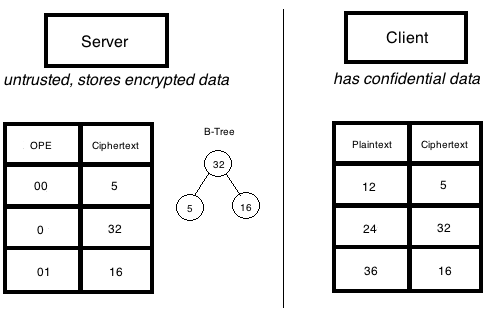
\includegraphics[height=4.2in,width=6in,angle=0]{857pic6.png}
\caption{The client hosts a series of plaintexts and their corresponding ciphertexts. The client provides the server with the ciphertexts, and the server maintains a B-tree ordered by plaintext values, along with a mapping between OPEs and ciphertexts.}
\end{center}
\end{figure}

\subsection{Protocol for Maintaining Order on Server}

As stated previously, the server orders the values in the B-tree based on plaintexts without knowing the plaintexts themselves. The server's ability to do so is best illustrated by considering how new values are added to the server's table by the client. In Figure 3 below, we consider the situation in which the client adds a new plaintext with value 30 and corresponding ciphertext with value 10 to the existing data from Figure 2.

To insert the value, the client first notifies the server, which subsequently gives back the client the ciphertext of the root node, which is 32. The client decrypts the ciphertext to find the corresponding plaintext, which has value 24, and subsequently determines whether the new plaintext he wishes to insert should lie to the right or left of the node returned by the server in order to preserve plaintext-based order in the B-tree. The client relays the proper direction to the server, which in this instance is the right side, and the server thereby moves right down the tree and gives the client the ciphertext of the right child of the root node. This interactive protocol continues until the server is unable to give the client a child node at the end of a tree path, and the client subsequently tells the server to add the new node to the appropriate postiion as a child of the existing leaf node. In this instance, the node with ciphertext 30 is inserted to the left of the node with ciphertext 16 since the ciphertext 30 has a plaintext with value 10, which is less than the plaintext with value 36 corresponding to the node with ciphertext of value 16. 

\begin{figure}[htb]
\begin{center}
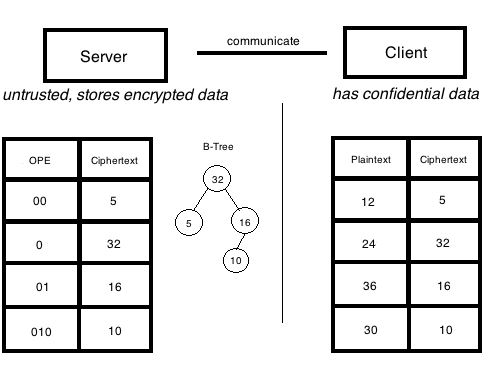
\includegraphics[height=4.5in,width=6in,angle=0]{857pic5.png}
\caption{The server is able to order the B-tree by the plaintext values of the nodes using an interactive protocol with the client.}
\end{center}
\end{figure}

\subsection{Handling repeated values}

When the client inserts multiple instances of the same value into the B-tree, the server does not create a new node for each such repeated value. Instead, the server provides only one node for a given plaintext value, and increments this count whenever the same value is added to the B-tree by the client. Unfortunately, this provides the server the ability to learn about the distribution of values in the B-tree based on the location and magnitute of node counts, and is the primary issue that the remaining portion of this paper addresses. 

\subsection{Related Work}

The mOPE scheme by Popa et al (2013) is the first scheme to achieve ideal IND-OCPA security, and our schemes are built upon mOPE. Further, Popa et al (2013) provides a new security definition, same-time OPE security, which dictates that an adversary can learn the order only for values stored in the application at the same time, and is stronger than IND-OCPA. Our security guarantee of IND-CPDA, explained later in the paper, asks furthermore that the ciphertexts not leak the distribution of values. Thus, our two schemes provide both same-time OPE security and IND-CPDA security.

Prior work in the field of OPE schemes falls short of providing IND-OCPA, proposed by Boldyreva et al (2009). Boldyreva et al (2009) prove that no immutable scheme can achieve IND-OCPA, however, Popa et al (2013) prove that IND-OCPA is in fact achievable with mutable ciphertexts, as described in the procedure above. The security alternative that Boldyreva et al (2009) present is that of random order-preserving function (ROPF). ROPF asks that an OPE scheme look "as-random-as-possible", while preserving order, and Boldyreva et al (2009) provide an OPE scheme that satisfies the notion of ROPF based on a random order-preserving function. However, OPE schemes that fall under the ROPF notion have been shown to leak at least half of the plaintext bits, in addition to order.

Prior work on range query schemes all leak information about the underlying plaintext. Shi et al (2007) designed an encryption scheme that encrypts the summaries of encrypted data, such that an authority may decrypt summaries that fall within a specific range. This scheme leaks the decrypted data for values that fall within the range query, but preserves the privacy of all other values. There is a tradeoff here, as for range queries under OPE schemes, one peice of information can be leaked for every value - the order - while in Shi et al's (2007) scheme, decrypted values are leaked, but nothing beyond the range query. We chose to build our schemes upon mOPE, instead of range query schemes, to guarantee that security of underlying plaintext. However, it would be interesting to explore the layering of range query schemes with OPE schemes to protect both the order and plaintext values.

\section{Distribution Confidentiality Scheme}

In order to solve the problem of leaking the distribution of the plaintext values, we have developed the Distribution Confidentiality Scheme (DCS). This scheme uses Popa et al (2013)'s original mOPE scheme, but adds an additional layer of security. We show that the schemes are comprable in terms of performance.

In essence, the DCS scheme adds random bits to the end of a plaintext so that the ciphertext values are randomized. This will prevent the server from being able to identify the number of times a repeated plaintext value is inserted.

\subsection{Description of DCS}

This section will give a formal description of DCS. We will first describe the basic version of the scheme, then we will augment it so that decimal numbers can be represented as well.

In the basic version of the scheme, let us assume that we want to encrypt some plaintext value $x \in \mathrm{Z}$ and send it to the server like in the mOPE scheme. For DCS, there is an additional parameter $\rho$ which will govern the probability with which the server sees a repeated value. We will generate a random value $r \in [0,1)$ which contains $\rho$ bits, denoted $r_{\rho}$, and append it to the end of $x$. The resulting value $x' = x + r_{\rho}$ will be encrypted with DET (a deterministic encryption algorithm, whose secret key $SK$ is held by the client but not the server). The mOPE scheme will work the same as before, but now acting on $x'$.

\subsection{Arbitrarily Small Collision Probability}

In this scheme, the probability of any ciphertexts being the same is small, and can be made arbitrarily close to zero by picking a larger $\rho$ parameter. In particular, the probability of any ciphertexts being the same is equivalent to the probability of any of the chosen random numbers $r$ being the same for two different encodings of some plaintext $x$.

Notice that this is exactly the birthday paradox problem since we must solve for the probability that any collision occurs. There are $2^\rho$ possible random numbers to be chosen. Now suppose that some value $x$ has $R(x)$ repetitions at the server, each with a plaintext value of $x'_i = x + r_i$ for the $i$th repetition. The probability of a collision and therefore a repeated ciphertext is just one minus the probability of no collisions:
\begin{eqnarray}
  Pr[\textrm{Ciphertext Collision of } Encode(SK, x)] = \prod_{i=1}^{R(x)} \left(1 - \frac{i}{2^{\rho}} \right)
\end{eqnarray}

The above expression is obtained because each newly chosen value $r_{i+1}$ can collide with $i$ previous values, out of the $2^{\rho}$ possible choices of $r_{i+1}$. Moreover, we can show that as $\rho \to \infty$, we obtain perfect collision protection. \\

\begin{lemma}
  If there exists some $N$ for which all $\rho > N$ have the property $R(x) \leq 2^{\rho}$ for all $x$ inserted into a DCS server tree, then as $\rho \to \infty$ the probability of collision approaches $0$.
\end{lemma}
\begin{proof}
  The probability of collision approching 0 is equivalent to showing that the probability of no collisions approaches one. We have shown that the probability of no collisions is:
  \begin{eqnarray}
    \prod_{i=1}^{R(x)} \left(1 - \frac{i}{2^{\rho}} \right) &\leq& \prod_{i=1}^{R(x)} \left(1 - \frac{R(x)}{2^{\rho}} \right) \\
                                                    &=& \left(1 - \frac{R(x)}{2^{\rho}} \right)^{R(x)}
  \end{eqnarray}

  Taking the limit as $\rho \to \infty$ and noting that $R(x) \leq 2^{\rho}$ for all $\rho > N$ so that $\lim_{\rho \to \infty} R(x) / 2^{\rho} = 0$, then we have:
  \begin{eqnarray}
    \lim_{\rho \to \infty} \left(1 - \frac{R(x)}{2^{\rho}} \right)^{R(x)} = 1
  \end{eqnarray}

  This shows that the collision probability approaches 0.
\end{proof}

Moreover, one can find an upper bound on the collision parameter $\rho$ one needs in order to not have collisions by using the upper bound of $(1 - R(x)/2^{\rho})^{R(x)}$ on the probability of no collisions. Setting this equal to one, we obtain:
\begin{eqnarray}
  \left(1 - \frac{R(x)}{2^{\rho}} \right)^{R(x)} &=& 1 \\
                                            \rho &=& \log_2 R(x)
\end{eqnarray}

Thus, choosing the correct $\rho$ to use is as simple as taking $y = \max_x R(x)$ over all input plaintext values $x$, and setting $\rho = \log_2 y$. Unfortunately, it may not be possible to predict $y$ ahead of time before insertions, and in any case, it would be nice to have a dynamic way of changing $\rho$ to the specifications of the problem.

\subsection{Dynamic Version of DCS}

To do this, we change the procedure of DCS slightly so that $\rho$ varies with $R(x)$. Note that the change we shall posit in this subsection does not change the insertion or querying mechanisms (to be discussed in the next subsections) and is purely an optimization.

The dynamic scheme will have a new collision parameter $\rho_x$ for each plaintext value $x$. We shall keep the invariant that $\rho_x \geq \log_2 R(x)$ at all times. We shall also keep a count of the number of times that $x$ has been repeated so far, $R(x)$, in an encrypted block of data on the server. Note that this encrypted block will be placed among numerous other data blocks that hold extra information. These data blocks are accessed directly by the client and will store data that cannot fit onto a single ciphertext from the mOPE encoding tree. The ciphertext blocks from the mOPE tree operate much like inodes in the UNIX filesystem, storing a pointer to the location of the relevant data blocks on the server. Each ciphertext in the mOPE tree which encrypts the plaintext $x' = x + r_i$ will store the location of the block containing $R(x)$.

This allows the client to access $R(x)$ whenever he queries for $x$. Thus, when attempting to insert some value $x$ into the mOPE tree, the client must first query for $x$ (the process of this will be discussed later), and check the current value of $R(x)$, and increment it on the encrypted block stored on the server. Then, the client will select a value $\rho_x \geq \log_2 R(x)$ and use this to construct the random value $|r| = 2^{\rho_x}$ and the ciphertext $c = Encrypt(SK, x + r)$. Insertion will then proceed normally.

Note that the ciphertext size for the mOPE tree must be fixed to some constant and that plaintext values will have to be padded. If there is no padding, then the adversary would be able to gain information on to the distribution of different repeated values with the same $\rho_x$ values. Note that arbitrarily long $\rho_x$ values can be used by simply using a linked list of encrypted data blocks on the server to store some ciphertext $c$ (although this would obviously negatively impact performance). All that is left to show is that collisions happen with low probability. \\

\begin{proposition}
  If one sets $\rho_x = c \lfloor \log_2 R(x) \rfloor$, then the probability of a collision is less than $2^c/R(x)^{c-1}$.
\end{proposition}
\begin{proof}
  We will proceed by induction. When $R(x) = 0$, this is trivially true since the next item inserted will never collide. Now, suppose it holds true for $R(x) = k$. We shall show that the $k+1$st insertion will collide with probabability less than $1/R(x)^{c-1}$.

  There are two cases when we insert $x$ the $k+1$st time. First, it could be that the collision parameter $\rho_x$ has increased, or in other words $\rho_x = c \lfloor \log_2 k + 1 \rfloor > c \lfloor \log_2 k \rfloor$. If this is the case, then the only way that a collision can happen with a previous value is if the first $c \lfloor \log_2 k \rfloor$ bits are the same as a previously held value, and the last $c \lfloor \log_2 k + 1 \rfloor - c \lfloor \log_2 k \rfloor$ bits are zeros. This would induce a collision in the scheme and happens with probability $R(x) / 2^{\rho_x}$ since there are $R(x)$ different ways that a previously held value to be followed by zeros can occur, out of the possible $2^{\rho_x}$ values.

  The second case is when the collision parameter $\rho_x$ does not increase. In this case, we need to not collide with the $R(x)$ existing values. A collision will occur with probability $R(x) / 2^{\rho_x}$, since there are $2^{\rho_x}$ possible choices and $R(x)$ values to collide with.

  Therefore, we see that the probability of collision in either case is:
  \begin{eqnarray}
    Pr[\textrm{Collision}] = \frac{R(x)}{2^{\rho_x}} &=& \frac{R(x)}{2^{c \lfloor \log_2 R(x) \rfloor}} \\
                                                     &\leq& \frac{R(x)}{2^{c \log_2 R(x) - c}} \\
                                                     &=& \frac{2^c}{R(x)^{c-1}}
  \end{eqnarray}

  This completes the proof.
\end{proof}

Therefore, choosing $c$ large enough will work for all values of $R(x)$, and will get better and better as $R(x)$ grows. To combat the fact that this probability is close to 1 when $R(x)$ is small, one can simply initialize $\rho_x$ to a larger value than the base case of 1, which makes the probability of collision early on very small. Continuing and adding more repetitions of a value $x$ only decreases the probability of collision. For instance, when $c = 5$, the probability of collision is around 5\% for 5 repeated inputs, but falls off dramatically to 0.3\% for 10 repeated inputs.

Using a rule like the one used in the above proposition should give a good dynamic scheme for $\rho_x$ which provides low probability of collision.

\subsection{Inserting in DCS}

Inserting in this scheme is simple, since nothing else has to be changed from the mOPE scheme. The client will take the value $x$ to insert, create $x'$, then encrypt $x'$ to obtain a ciphertext. Inserting this ciphertext will involve moving down the server's binary search tree. The insertion process is started by the client acquiring the root node. The client then checks to see if $x'$ is larger or smaller than the root's decrypted value. This informs the client as to the direction in which it should move. Once it arrives at a leaf node, the client will insert the new ciphertext in the correct direction. Figure \ref{insertion_figure} provides pseudocode for how one might create an insertion algorithm at the client.

\begin{figure}[htb]
\lstset{language=Python}
\begin{lstlisting}[frame=single]
class Client:
    def insert(x):
        r = random()
        xprime = x + r
        c = encrypt(client.secret_key, xprime)
        root_ciphertext = server.get_root()
        tree_moves(xprime, c, root_ciphertext)

    def tree_moves(value, encrypted_value, ciphertext):
        plaintext = decrypt(server.secret_key, ciphertext)
        if value < plaintext:
            new_ciphertext = server.move_left()
        elif value > plaintext:
            new_ciphertext = server.move_right()
        else:
            return server.insert(encrypted_value)
        tree_moves(value, encrypted_value, new_ciphertext)
\end{lstlisting}
\caption{Pseudocode for the Insertion Algorithm. The algorithm is a communication between the client and the server. The client asks for ciphertexts stored on the server, decrypts the ciphertexts, then determines whether to move left or right.}
\label{insertion_figure}
\end{figure}


\subsection{Querying Under DCS}

To query for some value $y$, we must actually perform a range query, since any value $y$ will be encrypted with a plaintext $y + r$ where $r \in [0,1)$. Therefore, the encrypted plaintext of $y$ can be in the range $[y, y + 1)$. Thus, to query for the value $y$, we must perform a range query on any values in the range $[y, y+1]$. The client will remove all values which are exactly equal to $y + 1$, but this should be arbitrarily small (in fact the probability will be $2^{-\rho}$ where $\rho$ is the collision parameter) so it should not affect performance in practice. Because of this, we shall abuse notation and say the process of querying the range $[y, y+1]$ and removing all values of $y+1$ will be equivalent to just querying the range $[y, y+1)$.

Performing this range query on the binary search tree can be done by searching for $y$ and $y+1$ individually. Once we have found $y$ and $y+1$, then we can move up the tree until we find the least common ancestor between the nodes of $y$ and $y+1$. The subtree rooted at the least common ancestor will contain all possible values in the range $[y, y+1)$. \\

  \begin{lemma}
    The subtree rooted at the least common ancestor of $y$ and $y+1$ in a binary search tree contains all values $x \in [y, y+1)$.
  \end{lemma}
  \begin{proof}
Let us examine some value $x \in [y, y+1)$, and call the $l$ the least common ancestor of $y$ and $y+1$. \\ \\
Now suppose $x$ is not in the subtree rooted at $l$. This means that $x$ must either be smaller than the left-most node in the subtree rooted at $l$ or greater than the right-most node in the subtree (assuming that no nodes are have repeated values, which occurs with high probability because of the random bits $r$ appended to each plaintext). However, we know that the left-most node in the subtree rooted at $l$ must be smaller than $y$ and the right-most node in the subtree must be greater than $y+1$. This is true because both $y$ and $y+1$ are nodes in the subtree. \\ \\
This is a contradiction, however, because we assumed $x \in [y, y+1)$, which shows that the subtree contains all values $x \in [y, y+1)$.
\end{proof}

This lemma instructs us on how to find all values $x \in [y, y+1)$. As we move up the binary search tree to parents of $y$, we check the right subtree of the parent looking for all values in $[y, y+1)$. We do this as we continue upwards for all successive parent nodes. For the node at $y+1$, we check the left subtree of all parents for values in $[y, y+1)$. We continue this process until the parent of the $y$ node meets the parent of the $y+1$ node. This process will find and return all values in $[y, y+1)$, because as we have shown, all values in the interval are inside the subtree. \\ \\
This process is correct because we continue checking subtrees until we find the least common ancestor for the parents of both the $y$ and the $y+1$ nodes. The runtime of this is just $\log(n) + K$ where $K$ is the number of values in the range $[y, y+1)$.

  \subsection{Range Queries Under DCS}

  To perform range queries under the DCS scheme, one simply needs to perform a range query on the underlying binary search tree. If one attempts to query for values $x \in [y, z]$, then we simply perform a range query for the underlying plaintexts in the binary search tree in the range $[y, z+1)$. We use the same range query mechanism as in the previous section, making sure to only output values that are inside in the interval $[y, z+1)$.
\section{Indistinguishability Under Chosen Plaintext Distribution Attack (IND-CPDA)}
This security definition consists of two phases of interaction between the adversary and the challenger. \\ \\
In phase I:
\begin{itemize}
  \item Client generates $SK \leftarrow KeyGen(1^\kappa)$ based on security parameter $\kappa$.
  \item Adversary may perform encryptions and other operations in time $poly(\kappa)$.
  \item Client chooses $b \leftarrow \{0,1\}$ uniformly at random (which the adversary does not know about).
\end{itemize} 

In phase II, the client and server engage in $poly(\kappa)$ rounds of interaction in which the adversary is adaptive. In each round $i$:
\begin{itemize}
  \item Adversary sends sequences $V_i^0, V_i^1 \in D^{\lambda}$ to the client each of size $\lambda$, where $\lambda$ is a fixed value, and $V_i = \{ v_{ij} \}_i^{\lambda}$ where $v_{ij}$ is the $j$th value chosen for round $i$.
  \item The client leads the interaction for the encryption algorithm on inputs $SK$ and $V_i^b$ with the server, with the adversary observing all the state at the server.
\end{itemize} 

In phase III:
\begin{itemize}
  \item Adversary obtains $poly(\lambda, \kappa)$ time to compute.
  \item Adversary outputs $b'$ as its guess for $b$. 
\end{itemize} 

The adversary shall win the game if its guess is correct $b' = b$ and the sets have the same order relations (namely that $v_{ij}^0 < v_{ik}^0 \Leftrightarrow v_{ij}^1 < v_{ik}^1$). 

\begin{definition}
  The adversary's advantage is the difference $|Pr[\textrm{win}^{Adv, \kappa, \lambda}] - 1/2|$.
\end{definition}

\begin{definition}
  IND-CPDA. A mOPE scheme is IND-CPDA secure if for all adversaries and all sufficiently large $\kappa$ and $\lambda$, the adversary's advantage is negligible, i.e. that $Pr[\textrm{win}^{Adv, \kappa, \lambda}] \leq 1/2 + \textrm{negl}(\kappa, \lambda)$.
\end{definition}

\subsection{Security of DCS}

\begin{theorem}
  DCS is IND-CPDA secure. 
\end{theorem}
\begin{proof}
We shall show that encrypting $v = \{V_1, V_2, \ldots, V_{\kappa} \}$ and $w = \{W_1, W_2, \ldots, W_{\kappa}\}$ is information-theoretically the same, where $V_i, W_i$ are sequences of size $\lambda$.

We will show this by induction on the number of repeated elements in either $V_i$ or $W_i$. We shall first consider the base case when there are no repeated elements in $V_i$ or in $W_i$, so that all the elements in $V_i$ are distinct, as well as the elements in $W_i$. In this case, the sequence $v$ can be broken down into $\kappa$ sequences of all distinct elements. This has a clear bijection to a sequence of elements $v_{ij}$ of length $\kappa \lambda$, for $i \in \{1, 2, \ldots, \kappa\}$ and $j \in \{1, 2, \ldots, \lambda \}$. Winning this game then becomes equivalent to winning the IND-OCPA security game, since one can think of each $v_{ij}$ and $w_{ij}$ pair as a set of values that the adversary provides the client in each round $i$. Popa et al (2013) show that their scheme, which is equivalent to the Distribution Confidentiality Scheme when there are no reptitions, is IND-OCPA secure. This means that the DCS scheme is IND-CPDA secure when there are no repeated elements.

Now we shall use strong induction and assume that when there are a maximum of $k$ repeated elements in both $V_i$ and $W_i$, the DCS scheme is IND-CPDA secure. To complete the proof, we simply need to show that when there are $k+1$ repeated elements, the DCS scheme is still secure.

Let us compare the sets $V_i$ and $W_i$ with $k+1$ repeated elements to the sets with $k$ repeated elements. In the $k+1$ case, there is one extra reptition with a value that has already appeared, on top of the $k$ repetitions that already exist. Now consider the plaintext $x$ which is repeated. The probability that the OPE encoding of $x$ has already appeared in the sequence of elements in the set $V_i$ or $W_i$ is negligible. Since the OPE encoding is not repeated by the new value $x$, the number of OPE encoding repetitions is at most $k$. However, we have shown that when there are $k$ repeated elements in the sets $V_i$ and $W_i$, then DCS is IND-CPDA secure by the inductive hypothesis. Since the largest number of repeated encodings in this case is $k$, this is the same situation as when there are $k$ repeated elements in the sets $V_i$ and $W_i$. Therefore, when there are $k+1$ repeated elements, DCS is IND-CPDA secure.
We have therefore shown by induction that DCS is IND-CPDA secure for any number of repeated elements in the sets $V_i$ and $W_i$, which completes the proof that DCS is IND-CPDA secure.
\end{proof}

\section{Random Tiebreaking Order Preserving Encryption (RTOPE)}

Consider another simple tie-breaking rule on top of the mOPE scheme. When the client inserts a new ciphertext $c^*$ into the server, the client proceeds normally when the ciphertext $c_i$ returned by the server does not get decrypted to a plaintext $p_i$ which is equal to $p^* = Dec(SK, c^*)$. However, if $p_i = p^*$, then the client tells the server to move left or right with uniform probability. Note that in this scheme, we will use a randomized encryption scheme which is IND-CCA so that the server cannot tell if two plaintext values are the same.

To query a ciphertext $c^*$, one needs to make sure to find all possible places where $c^*$ can exist. Thus, whenever the server returns $c_i$ which decrypts to $p_i = p^* = Dec(SK, c^*)$, then one must check both the left and right subtrees of $c_i$ to see if $c^*$ exists. Querying each subtree is done with the  normal Popa et al (2013) process.

This scheme is a simple extension of the mOPE scheme and handles repeated values. In RTOPE, the server cannot tell how many values are repeated, nor what distribution of repeated values looks like.

\subsection{Querying Under RTOPE}

Under RTOPE, there are multiple variations of querying for some value $x$. First is to query for just one ciphertext whose corresponding plaintext is equal to $x$. The second query type is to query for all ciphertexts whose corresponding plaintext is equal to $x$.

The first case is easy to handle and can be achieved by using the regular query mechanism used by Popa et al (2013) and returning the first ciphertext found which matches. If there are any ciphertexts which can be decrypted to $x$, then the regular binary search tree mechanism will find at least one, which guarantees that this will correctly return one of these ciphertexts.

The second case can be handled by a modified query algorithm. To return all ciphertexts decrypting to $x$, we still need to do a regular query for $x$. Upon finding the first $x$, we append this value to our list of results, and we need to query both the right and left subtrees for $x$ again. Doing this recursively until we reach a leaf will guarantee that we will find all possible places where $x$. This gaurantee can be given in the following proposition: \\ \\

  \begin{proposition}
    Let $T$ be a binary search tree and $x$ be a repeated value in the binary search tree. There exists a subtree $T'$ rooted at $x$ which contains all values $x$ in the tree $T$.
  \end{proposition}
  \begin{proof}
    We shall construct the tree by taking all possible values of $x$, and finding the lowest common ancestor of each of these values. It is always possible to find the lowest common ancestor of each of these values, and these will create a subtree. All that is left is to show that the subtree is rooted at $x$, or in other words, that the least common ancestor of all the values of $x$ in the tree is also $x$. \\ \\
We note that there are three cases. First, if $x$ is not repeated (i.e. occurs in the tree only once), then the proposition is trivially true. Second, if $x$ is repeated, and all the repeated values are in the right subtree of the least common ancestor, then one can choose the value of $x$ which has the largest height in the binary search tree. This defines a subtree containing all values of $x$ and which is also rooted at $x$. The same idea follows when all the repeated values of $x$ are in the left subtree. Finally, if the repeated values of $x$ are in both the left and right subtree of the least common ancestor $l$, then we know that $x \leq l$ and $x \geq l$ by the properties of a binary search tree. This implies that $l = x$, which completes the proof.
  \end{proof}

By the above proposition, we can show that as soon as we find the first value of $x$ based on the regular binary search tree query algorithm, then all other values of $x$ will be contained in either the left or right subtree of this node. This implies that we will find all values of $x$ in the tree.

The runtime $T(n)$ of this query can found by noting that in the worst case, every element in the tree is repeated so querying for $x$ will require $O(n)$ time. This is an extreme case, however, and it is more likely given by the relation:
\begin{eqnarray}
  T(n) = 2 T(n/2) + O(1)
\end{eqnarray}

Since if a node is found to be the same, then the problem is broken into two smaller problems on the left and right subtrees, which are both of size $O(n/2)$ for a balanced tree. The solution of this recurrence is $O(\log n)$, so one can usually expect a logarithmic running time.

  \subsection{Security of RTOPE}

  RTOPE can be proven to be IND-CPDA, just like the DCS scheme. \\

  \begin{theorem}
    RTOPE is IND-CPDA secure.
  \end{theorem}
  \begin{proof}
    Like in the security proof for DCS, we shall show that encrypting $v = \{V_1, V_2, \ldots, V_{\kappa} \}$ and $w = \{W_1, W_2, \ldots, W_{\kappa}\}$ is information-theoretically the same, where $V_i, W_i$ are sequences of size $\lambda$. Again, we shall use induction on the number of repeated elements in either $V_i$ or $W_i$. 

When there are no repeated elements, we can use the same argument we used in the DCS proof. We note that the sequence $\{V_1, V_2, \ldots, V_{\kappa} \}$ has a bijection to a sequence of elements $v_{ij}$ of length $\kappa \lambda$, for $i \in \{1, 2, \ldots, \kappa\}$ and $j \in \{1, 2, \ldots, \lambda \}$. Winning this game then becomes equivalent to winning the IND-OCPA security game, since one can think of each $v_{ij}$ and $w_{ij}$ pair as a set of values that the adversary provides the client in each round $i$. Popa et al (2013) shows that their scheme, which is equivalent to the Distribution Confidentiality Scheme when there are no repetitions, is IND-OCPA secure. Thus, the base case of no repetitions is secure.

Now, suppose that RTOPE is IND-CPDA secure when there are at most $k$ repetitions across $V_i$ and $W_i$. Now consider a sequence where there are $k+1$ repetitions across $V_i$ and $W_i$ for all $i$. Select two ciphertexts $c_1$ and $c_2$ of some repeated value $x$ and let us consider how this pair of repetitions is inserted into the tree. Since RTOPE uses an encryption scheme which is IND-CCA for its ciphertexts, the adversary will not be able to tell whether $Dec(SK, c_1) = Dec(SK, c_2)$ with more than $1/2$ probability (by the definition of IND-CCA security). This means that the adversary cannot distinguish $c_1$ and $c_2$ as being repetitions with any advantage. Thus, a sequence of $k+1$ repetitions is information theoretically the same for the adversary as a sequence of $k$ repetitions, which we already know is IND-CPDA secure. Using induction, we have completed the proof.
  \end{proof}

\section{Relationship Between DCS and RTOPE}

  In this section, we shall propose a notion of equivalence between two OPE schemes and examine whether DCS and RTOPE are equivalent.

  \subsection{Structural Expectation Equivalence} 

\begin{definition} 
  Two OPE schemes $x,y$ are \emph{Structural Expectation Equivalent} if for each plaintext $p_i$ that scheme $x$ encodes in a sequence of plaintexts $P = \{p_i\}_{i=1}^n$, there exists some bijective mapping $f: \mathrm{Z}_y \to \mathrm{Z}_x$ where $Pr[Encode_x(c_i) = \omega] = Pr[f(Encode_y(c_i)) = \omega]$ for all $\omega \in \mathrm{Z}_x$ where $\mathrm{Z}_x$ is the space of all possible OPE encodings for scheme $x$, $c_i = Enc(SK, p_i)$ is the ciphertext corresponding to $p_i$, and $Encode_x(c_i)$ and $Encode_y(c_i)$ are the functions that obtain the OPE encoding for schemes $x$ and $y$ respectively.
\end{definition}

In other words, for two schemes to be structurally expectation equivalent, there must exist a mapping $f$ from all of the possible OPE encodings from scheme $x$ to scheme $y$, where the probability of obtaining an encoding in $x$ is the same as the probability of obtaining the corresponding encoding in $y$ (based on the mapping). This must be the case for all possible encodings. \\ \\
This notion of structural expectation equivalence encompasses a number of useful features. In particular, notice that if $x$ is an OPE encoding scheme which is IND-CPDA secure, and $y$ is structurally expectation equivalent to $x$, then $y$ is also IND-CPDA secure. Due to this notion, it is sufficient to show the structural expectation equivalence of two schemes in order to link the IND-CPDA security of the schemes (the proof of this property is given in the theorem below). Another observation one can make is that the mapping in the structural expectation equivalence definition is bijective. Hence, if $x$ is structurally expectation equivalent to $y$, then $y$ is necessarily structurally expectation equivalent to $x$ because one can simply use $f^{-1}$ as the mapping, which necessarily exists because of $f$ being bijective. \\

\begin{theorem}
 If two OPE schemes $x,y$ are structurally expectation equivalent, then $x$ is IND-CPDA secure if and only if $y$ is IND-CPDA secure.
\end{theorem}
\begin{proof}
First, we observe that notion of equivalence is symmetric (since $f$ is a bijective mapping which is invertible), so that without loss of generality, we need only show that if $x$ is IND-CPDA secure, then $y$ is as well. So now we can suppose that $x$ is IND-CPDA secure and $x,y$ are equivalent schemes.

Since $x$ is IND-CPDA secure, then for any two sequences $v = \{V_1, V_2, \ldots, V_{\kappa}\}$ and $w = \{W_1, W_2, \ldots, W_{\kappa} \}$ that the adversary provides to scheme $x$, the adversary cannot correctly distinguish between $v$ and $w$ with non-neglible advantage. Now suppose by contradiction that $y$ is not IND-CPDA secure. Then there exist two sequences $v' = \{V_1', \ldots, V_{\kappa}'\}$ and $w' = \{W_1', \ldots, W_{\kappa}'\}$ of plaintexts that the adversary can provide to the client in scheme $y$ so that he can distinguish the two sequences with non-neglible advantage in the client-server interaction. This means that the adversary can distinguish the encoding $Encode_y(V_i') = \{Encode_y(V_{ij}') \}_{j=1}^{\lambda}$ for some $i$ from the encoding $Encode_y(W_i') = \{Encode_y(W_{ij}') \}_{j=1}^{\lambda}$.

This means the adversary can also distinguish the mapping $Encode_x(V_i')$ from the encoding $Encode_x(W_i')$ by applying the bijective mapping $f$ (from the definition of equivalence) to obtain $Encode_x(V_i') = f(Encode_y(V_i'))$ and $Encode_x(W_i') = f(Encode_y(W_i'))$. This is a contradiction because it shows that $x$ is not IND-CPDA secure, which was one of our assumptions. Thus, we see by contradiction that $y$ must be IND-CPDA secure, which proves our result.
\end{proof}

\subsection{Structural Expectation Equivalence of DCS and RTOPE}

In this section, we shall investigate whether DCS and RTOPE are structurally expectation equivalent. To do this, we shall first examine some propositions. \\

\begin{proposition}
 There exists some subtree which contains all the ciphertexts corresponding to a plaintext $x$ in both DCS and RTOPE.
\end{proposition}
\begin{proof}
  This proposition is immediately clear because one can always take the entire tree as the subtree. This works for the ciphertext trees stored in both DCS and RTOPE.
\end{proof}

Since a subtree containing all the ciphertexts corresponding to a plaintext $x$ exists, we can now examine properties of this subtree. First, we show that the root of the smallest possible such subtree must be a ciphertext which gets decrypted to $x$. \\

\begin{proposition}
  The smallest subtree containing all ciphertexts which can be decrypted to some plaintext $x$ is rooted at a ciphertext $c$ such that $x = Dec(SK, c)$ in both DCS and RTOPE.
\end{proposition}
\begin{proof}
  First, we know that a subtree containing all ciphertexts which can be decrypted to $x$ exists, by the proposition we gave above. We therefore also know that a smallest subtree exists because the entire tree is of finite size. Now we shall show that this smallest subtree is rooted at $c$ such that $x = Dec(SK, c)$ for DCS. \\ \\
Suppose not, by contradiction. Then some ciphertext $c'$ is at the root such that $x' = Dec(SK, c')$ where $x' \neq x$. Since DCS is normalized to integer plaintexts, we must have $|x' - x| \geq 1$. We know, moreover, that there must be at least one ciphertext $c_l$ in the left subtree of the root and $c_r$ in the right subtree of the root such that $x = Dec(SK, c_l) = Dec(SK, c_r)$. If not, then the subtree we are in is not the smallest subtree containing all ciphertexts which decrypt to $x$ because one can simply take either the right or left subtree (depending on if the left or right subtree does not contain $c_l$ or $c_r$ respectively). \\ \\
However, we know that $Dec(SK, c_l) \leq Dec(SK, c') \leq Dec(SK, c_r)$ by the fact that $c_l$ is in the left subtree of $c'$ and that $c_r$ is in the right subtree. This implies that $x \leq x' \leq x$ so that $x' = x$. However, this is a contradiction because we assumed that $x' \neq x$. We have therefore shown that for DCS, the smallest subtree containing all cipertexts decrypting to $x$ must be rooted at a ciphertext decrypting to $x$. \\ \\
The proof for RTOPE is similar and we only provide a sketch. If $c'$ is a root which does not decrypt to $x$, then it must be separating a left and right subtree which contain $c_l$ and $c_r$, respectively, which decrypt to $x$. This means that $Dec(SK, c_l) \leq Dec(SK, c') \leq Dec(SK, c_r)$ which means that $x' = x$, which results in a contradiction (just like in the proof for DCS).
\end{proof}

We have seen that the smallest subtree containing a repeated plaintext will be rooted at a ciphertext decrypting to that plaintext. This has a number of interesting applications. For instance, one can examine the series of decisions that are made in the RTOPE scheme by the client by examining this subtree and a smaller subtree in a recursive fashion. \\ \\
For DCS, one can see that moving left or right from the root element depends on the relative size of the root element with the new element being inserted or queried. For example, if $x$ is the value of a repeated plaintext, then DCS will mutate $p$ into $p + r$ where $r \in [0,1)$ are some random bits. Moving left at the root means that $p_1 < p_r$ where $p_r$ is the root value. This means that $p + r_1 < p + r_r$, which is equivalent to saying $r_1 < r_r$. Thus, moving left at the root is just the probability that the random number $r_1$ is smaller than the random number $r_r$ picked at the root. \\ \\
Now let us examine some series of moves down the tree when attempting to query or insert some node with plaintext value $x$, denoted by the sequence
  \begin{eqnarray}
    \{ m_0(x), m_1(x), \ldots, m_k(x) \}
  \end{eqnarray}
We shall drop the $x$ for convenience and commonly refer to moves as $m_i$. We see that $m_i$ can take on two possibilities, 0 for left or 1 for moving right, and we can characterize the moves:
  \begin{eqnarray}
    m_i(x) = \left\{ \begin{array}{l l}
        0 & \textrm{if } p_i > x \\
        1 & \textrm{else}
    \end{array} \right.
  \end{eqnarray}

Here $p_i$ is the underlying plaintext value of the node at the $i$th move. We shall proceed to show that the two schemes do not produce the same expected tree. \\
\begin{theorem}
    DCS and RTOPE are not structurally expectation equivalent.
  \end{theorem}
  \begin{proof}
We shall prove this theorem by examining a sequence of moves when looking at the insertion of a repeated value $x$. In DCS, to move right so that $m_i = 1$, one must have $p_i < x + r$. To move left, one must have $p_i > x + r$. Although there exists a sequence of moves from the root to a leaf of the tree which includes every node in the tree, we need only examine the nodes which have a plaintext value equal to $x$ (before the addition of the random bit). This is because the traversal of DCS and RTOPE is the same for nodes which are not repeated (they share the normal binary tree traversal rule). Thus, we know that the moves in these cases will be equivalent and the probability of making the moves on non-repeated nodes will be equal.

Thus, we can reduce our problem to considering a sequence of moves \{$m_i\}_{i=1}^k$ on the plaintext values which are equal to $x$. By the propsition we proved above, this sequence of moves will be rooted at a ciphertext which is an encrypted value of $x$. Making any sequence of moves on repeated values in RTOPE will have probability $2^{-k}$ where $k$ is the number of repeated value in the sequence down the tree. This is becase one moves left or right with probability $\frac{1}{2}$.

Now we shall examine the sequence of moves in DCS. Recall that we need only consider a sequence of moves $\{m_i\}_{i=1}^k$ which is performed on a single repeated plaintext value $x$. This means that in DCS, the plaintext values will be distinguished by the random bit $r_i$ so that $p_i = x + r_i$. Therefore, we need only compare $r_i$ to the value $r^*$, where $r^*$ is the random part of the new plaintext we are inserting.

The probability that we make a series of moves $\{m_i\}_{i=1}^k$ is the probability that $r^*$ has the $j$ and $j+1$st smallest elements in the sequence of random values $\{ r_i\}_{i=1}^k$. Let $n = R(x)$ be the total number of repeated values of $x$.

It is well known that the probability that the $j$th smallest element falling in the interval $[u, u + du]$ is given by:
    \begin{eqnarray}
      \frac{n!}{(j-1)!(n-j)!} u^{j-1} (1-u)^{n-j} du
    \end{eqnarray}

Therefore, the probability that $r^*$ falls between the $j$th and $j+1$st value is just the difference between all potential values $u_1$ of the $j$th smallest element and all potential values $u_2$ of the $j+1$st element. This is:
    \begin{eqnarray}
      \int_{0}^1 \int_0^{u_2} Pr[U_2 = u_2] Pr[U_1 = u_1] Pr[u_1 < r^* < u_2] d_{u_1} d_{u_2}
    \end{eqnarray}

Where we take $U_1$ as the $j$th smallest value and $U_2$ as the $j+1$st smallest value. Thus, the probability of $r^*$ falling in that interval is the integral over all possible values of $U_2$ and $U_1$, and the probability that it falls inside of the that interval. Since $Pr[u_1 < r^* < u_2] = (u_2 - u_1)$, we can write the above as:
\begin{eqnarray}
      \int_{0}^1 \int_0^{u_2} \left( \frac{n!}{j!(n-j-1)!} u_2^j (1 - u_2)^{n-j-1} \right) \left( \frac{n!}{(j-1)!(n-j)!} u_1^{j-1} (1 - u_1)^{n-j} \right) (u_2 - u_1) d_{u_1} d_{u_2}
    \end{eqnarray}

Letting $C(j) = \frac{n!}{j!(n-j-1)!} \frac{n!}{(j-1)!(n-j)!}$, and integrating the expression for $u_1$, we can obtain the following result:
    \begin{eqnarray}
      C(j) \int_0^1 u_2^j (1 - u_2)^{n-j-1} \left( \frac{(u_2 (n+1) - j) B(j, n-j+1) + u_2^j (1-u_2)^{n-j+1}}{n+1} \right) d u_2
    \end{eqnarray}

The above is the probability that $r^*$ falls between the $j$th and $j+1$st values. Simulating this in the figure below, it is clear that this is not uniform for all values of $j$ (like RTOPE is).
    \begin{figure}[H]
      \centering
      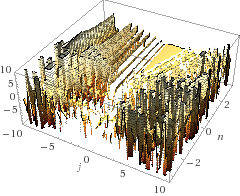
\includegraphics[width=3in]{ball_result.png}
      \caption{Probability of $r^*$ falling between the $j$th and $j+1$st largest values in the sequence $\{r_i\}_{i=1}^n$}
    \end{figure}

  We have therefore shown that DCS and RTOPE are not structurally expectation equivalent.
  \end{proof}

\section{Experimental Results}

To confirm our theoretical analysis, we implemented both the DCS and RTOPE encryption schemes on top of a simplified client server interface (like the one Popa et al (2013) used). First, we created a framework that mimicked the necessary features of an mOPE, including the client-server interaction and full insertion and query functionality. We then made a testing framework which allowed us to easily change the number of inputs, the number of repeats in the inputs, and the choice of whether to use DCS or RTOPE. The results are summarized in the table \ref{tab:results_table}.

\begin{table} % Add the following just after the closing bracket on this line to specify a position for the table on the page: [h], [t], [b] or [p] - these mean: here, top, bottom and on a separate page, respectively
\centering % Centers the table on the page, comment out to left-justify
\begin{tabular}{l c c c c} % The final bracket specifies the number of columns in the table along with left and right borders which are specified using vertical bars (|); each column can be left, right or center-justified using l, r or c. To specify a precise width, use p{width}, e.g. p{5cm}
\toprule % Top horizontal line
& \multicolumn{4}{c}{Number of OPE Re-Encodings} \\ % Amalgamating several columns into one cell is done using the \multicolumn command as seen on this line
\cmidrule(l){2-5} % Horizontal line spanning less than the full width of the table - you can add (r) or (l) just before the opening curly bracket to shorten the rule on the left or right side
Type & Inputs & Repeats & Average & Std. Dev.\\ % Column names row
\midrule % In-table horizontal line
RTOPE & 100 & 0  & 7363 & 5003 \\
      & 100 & 10  & 4385 & 2051 \\
      & 100 & 20  & 3945 & 643\\
      & 100 & 40  & 2598 & 642\\
      \midrule
DCS   & 100 & 0  & 3776 & 791 \\
      & 100 & 10  & 4452 & 1059 \\
      & 100 & 20  & 3287 & 1191\\
      & 100 & 40  & 3754 & 582\\
      \midrule
RTOPE & 200 & 0  & 15078 & 6751 \\
      & 200 & 20  & 16586 & 13215\\
      & 200 & 40  & 15707 & 6924\\
      \midrule
DCS   & 200 & 0  & 11300 & 2512 \\
      & 200 & 20  & 12355 & 8704\\
      & 200 & 40  & 8274 & 1654\\
\bottomrule % Bottom horizontal line
\end{tabular}
\caption{Experimental results. N=10 for each set of inputs.} % Table caption, can be commented out if no caption is required
\label{tab:results_table} % A label for referencing this table elsewhere, references are used in text as \ref{label}
\end{table}

Each iteration constructed an entire tree from random inputs fitting the input criteria. The averages and standard deviations describe the distribution of the number of OPE re-encodings required throughout the construction of the tree. We make several observations from the data:

\begin{enumerate}
\item For large inputs, the average number of OPE re-encodings is roughly the same for both schemes. We found that even though the two schemes are not identical, they do have the same expectation for the shape of the resulting trees over a large number of iterations, so the averages will be the same.
\item The standard deviation in OPE re-encodings varies significantly between the two schemes. This has to do with the resulting shape of the trees formed for the same inputs - DCS is more likely to create an unbalanced tree, and thus the standard deviations tend to be higher than comparable RTOPE deviations.
\item
The average number of OPE re-encodings is roughly the same for any number of repeated items. In DCS, each duplicate is converted into a unique number before the insertion phase. In RTOPE, each value is treated as if it were either larger or smaller than its duplicate during the insertion phase. In both cases, the server is not made aware of duplicate values, and thus their quantity has no bearing on the properties of the tree created by the server.
\end{enumerate}

\section{Conclusion}

 We presented DCS and RTOPE, two order-preserving encryption schemes that achieve ideal IND-CPDA security, where an adversary learns nothing about the distribution of the plaintext values based on the ciphertexts, and only the order of the elements. DCS generates random bits to append to any plaintext value that is encrypted, which requires a modified querying scheme involving localized range queries. RTOPE handles repeated values differently, by appending repeated plaintexts as left or right children on the server's search tree with uniform probability. Again, we created a modified querying algorithm for RTOPE that requires recursive queries once one occurence of the plaintext query is found. 

We proved that DCS and RTOPE are IND-CPDA secure and introduced the notion of structurally expectation equivalence. We also proved the important theorem that if two OPE schemes are structurally expectation equivalent, then one is IND-CPDA secure if and only if the other is IND-CPDA secure as well. We then showed that DCS and RTOPE do not satisfy this structurally expectation equivalence relationship.

We noted that though the schemes are not structurally expectation equivalent, the number of OPE re-encodings will converege to the same number, given identical inputs. This notion was supported by our experimental results, which we tested on a range of inputs.

\begin{thebibliography}{9}

\bibitem{adapopa13}
  R.A. Popa, F. Li, N. Zeldovich.
  An Ideal-Security Protocol for Order Preserving Encoding.
  2013.

\bibitem{boldyreva11}
  A. Boldyreva, N. Chenette, and A. O’Neill. 
  Order-preserving encryption revisited: improved security analysis and alternative
  solutions. \emph{CRYPTO}, 2011.
  
\bibitem{Shi07}
  E. Shi, J. Bethencourt, T.-H. H. Chan, D. Song, and A. Perrig.
Multi-dimension range query over encrypted data. In \emph{IEEE
Symposium on Security and Privacy}, 2007.

\end{thebibliography}
  

\end{document}
